
% Default to the notebook output style

    


% Inherit from the specified cell style.




    
\documentclass{article}

    
    
    \usepackage{graphicx} % Used to insert images
    \usepackage{adjustbox} % Used to constrain images to a maximum size 
    \usepackage{color} % Allow colors to be defined
    \usepackage{enumerate} % Needed for markdown enumerations to work
    \usepackage{geometry} % Used to adjust the document margins
    \usepackage{amsmath} % Equations
    \usepackage{amssymb} % Equations
    \usepackage{eurosym} % defines \euro
    \usepackage[mathletters]{ucs} % Extended unicode (utf-8) support
    \usepackage[utf8x]{inputenc} % Allow utf-8 characters in the tex document
    \usepackage{fancyvrb} % verbatim replacement that allows latex
    \usepackage{grffile} % extends the file name processing of package graphics 
                         % to support a larger range 
    % The hyperref package gives us a pdf with properly built
    % internal navigation ('pdf bookmarks' for the table of contents,
    % internal cross-reference links, web links for URLs, etc.)
    \usepackage{hyperref}
    \usepackage{longtable} % longtable support required by pandoc >1.10
    \usepackage{booktabs}  % table support for pandoc > 1.12.2
    \usepackage{ulem} % ulem is needed to support strikethroughs (\sout)
    

    
    
    \definecolor{orange}{cmyk}{0,0.4,0.8,0.2}
    \definecolor{darkorange}{rgb}{.71,0.21,0.01}
    \definecolor{darkgreen}{rgb}{.12,.54,.11}
    \definecolor{myteal}{rgb}{.26, .44, .56}
    \definecolor{gray}{gray}{0.45}
    \definecolor{lightgray}{gray}{.95}
    \definecolor{mediumgray}{gray}{.8}
    \definecolor{inputbackground}{rgb}{.95, .95, .85}
    \definecolor{outputbackground}{rgb}{.95, .95, .95}
    \definecolor{traceback}{rgb}{1, .95, .95}
    % ansi colors
    \definecolor{red}{rgb}{.6,0,0}
    \definecolor{green}{rgb}{0,.65,0}
    \definecolor{brown}{rgb}{0.6,0.6,0}
    \definecolor{blue}{rgb}{0,.145,.698}
    \definecolor{purple}{rgb}{.698,.145,.698}
    \definecolor{cyan}{rgb}{0,.698,.698}
    \definecolor{lightgray}{gray}{0.5}
    
    % bright ansi colors
    \definecolor{darkgray}{gray}{0.25}
    \definecolor{lightred}{rgb}{1.0,0.39,0.28}
    \definecolor{lightgreen}{rgb}{0.48,0.99,0.0}
    \definecolor{lightblue}{rgb}{0.53,0.81,0.92}
    \definecolor{lightpurple}{rgb}{0.87,0.63,0.87}
    \definecolor{lightcyan}{rgb}{0.5,1.0,0.83}
    
    % commands and environments needed by pandoc snippets
    % extracted from the output of `pandoc -s`
    \providecommand{\tightlist}{%
      \setlength{\itemsep}{0pt}\setlength{\parskip}{0pt}}
    \DefineVerbatimEnvironment{Highlighting}{Verbatim}{commandchars=\\\{\}}
    % Add ',fontsize=\small' for more characters per line
    \newenvironment{Shaded}{}{}
    \newcommand{\KeywordTok}[1]{\textcolor[rgb]{0.00,0.44,0.13}{\textbf{{#1}}}}
    \newcommand{\DataTypeTok}[1]{\textcolor[rgb]{0.56,0.13,0.00}{{#1}}}
    \newcommand{\DecValTok}[1]{\textcolor[rgb]{0.25,0.63,0.44}{{#1}}}
    \newcommand{\BaseNTok}[1]{\textcolor[rgb]{0.25,0.63,0.44}{{#1}}}
    \newcommand{\FloatTok}[1]{\textcolor[rgb]{0.25,0.63,0.44}{{#1}}}
    \newcommand{\CharTok}[1]{\textcolor[rgb]{0.25,0.44,0.63}{{#1}}}
    \newcommand{\StringTok}[1]{\textcolor[rgb]{0.25,0.44,0.63}{{#1}}}
    \newcommand{\CommentTok}[1]{\textcolor[rgb]{0.38,0.63,0.69}{\textit{{#1}}}}
    \newcommand{\OtherTok}[1]{\textcolor[rgb]{0.00,0.44,0.13}{{#1}}}
    \newcommand{\AlertTok}[1]{\textcolor[rgb]{1.00,0.00,0.00}{\textbf{{#1}}}}
    \newcommand{\FunctionTok}[1]{\textcolor[rgb]{0.02,0.16,0.49}{{#1}}}
    \newcommand{\RegionMarkerTok}[1]{{#1}}
    \newcommand{\ErrorTok}[1]{\textcolor[rgb]{1.00,0.00,0.00}{\textbf{{#1}}}}
    \newcommand{\NormalTok}[1]{{#1}}
    
    % Additional commands for more recent versions of Pandoc
    \newcommand{\ConstantTok}[1]{\textcolor[rgb]{0.53,0.00,0.00}{{#1}}}
    \newcommand{\SpecialCharTok}[1]{\textcolor[rgb]{0.25,0.44,0.63}{{#1}}}
    \newcommand{\VerbatimStringTok}[1]{\textcolor[rgb]{0.25,0.44,0.63}{{#1}}}
    \newcommand{\SpecialStringTok}[1]{\textcolor[rgb]{0.73,0.40,0.53}{{#1}}}
    \newcommand{\ImportTok}[1]{{#1}}
    \newcommand{\DocumentationTok}[1]{\textcolor[rgb]{0.73,0.13,0.13}{\textit{{#1}}}}
    \newcommand{\AnnotationTok}[1]{\textcolor[rgb]{0.38,0.63,0.69}{\textbf{\textit{{#1}}}}}
    \newcommand{\CommentVarTok}[1]{\textcolor[rgb]{0.38,0.63,0.69}{\textbf{\textit{{#1}}}}}
    \newcommand{\VariableTok}[1]{\textcolor[rgb]{0.10,0.09,0.49}{{#1}}}
    \newcommand{\ControlFlowTok}[1]{\textcolor[rgb]{0.00,0.44,0.13}{\textbf{{#1}}}}
    \newcommand{\OperatorTok}[1]{\textcolor[rgb]{0.40,0.40,0.40}{{#1}}}
    \newcommand{\BuiltInTok}[1]{{#1}}
    \newcommand{\ExtensionTok}[1]{{#1}}
    \newcommand{\PreprocessorTok}[1]{\textcolor[rgb]{0.74,0.48,0.00}{{#1}}}
    \newcommand{\AttributeTok}[1]{\textcolor[rgb]{0.49,0.56,0.16}{{#1}}}
    \newcommand{\InformationTok}[1]{\textcolor[rgb]{0.38,0.63,0.69}{\textbf{\textit{{#1}}}}}
    \newcommand{\WarningTok}[1]{\textcolor[rgb]{0.38,0.63,0.69}{\textbf{\textit{{#1}}}}}
    
    
    % Define a nice break command that doesn't care if a line doesn't already
    % exist.
    \def\br{\hspace*{\fill} \\* }
    % Math Jax compatability definitions
    \def\gt{>}
    \def\lt{<}
    % Document parameters
    \title{neki kao grafovi}
    
    
    

    % Pygments definitions
    
\makeatletter
\def\PY@reset{\let\PY@it=\relax \let\PY@bf=\relax%
    \let\PY@ul=\relax \let\PY@tc=\relax%
    \let\PY@bc=\relax \let\PY@ff=\relax}
\def\PY@tok#1{\csname PY@tok@#1\endcsname}
\def\PY@toks#1+{\ifx\relax#1\empty\else%
    \PY@tok{#1}\expandafter\PY@toks\fi}
\def\PY@do#1{\PY@bc{\PY@tc{\PY@ul{%
    \PY@it{\PY@bf{\PY@ff{#1}}}}}}}
\def\PY#1#2{\PY@reset\PY@toks#1+\relax+\PY@do{#2}}

\expandafter\def\csname PY@tok@kn\endcsname{\let\PY@bf=\textbf\def\PY@tc##1{\textcolor[rgb]{0.00,0.50,0.00}{##1}}}
\expandafter\def\csname PY@tok@ow\endcsname{\let\PY@bf=\textbf\def\PY@tc##1{\textcolor[rgb]{0.67,0.13,1.00}{##1}}}
\expandafter\def\csname PY@tok@nt\endcsname{\let\PY@bf=\textbf\def\PY@tc##1{\textcolor[rgb]{0.00,0.50,0.00}{##1}}}
\expandafter\def\csname PY@tok@ss\endcsname{\def\PY@tc##1{\textcolor[rgb]{0.10,0.09,0.49}{##1}}}
\expandafter\def\csname PY@tok@se\endcsname{\let\PY@bf=\textbf\def\PY@tc##1{\textcolor[rgb]{0.73,0.40,0.13}{##1}}}
\expandafter\def\csname PY@tok@gs\endcsname{\let\PY@bf=\textbf}
\expandafter\def\csname PY@tok@il\endcsname{\def\PY@tc##1{\textcolor[rgb]{0.40,0.40,0.40}{##1}}}
\expandafter\def\csname PY@tok@kp\endcsname{\def\PY@tc##1{\textcolor[rgb]{0.00,0.50,0.00}{##1}}}
\expandafter\def\csname PY@tok@gu\endcsname{\let\PY@bf=\textbf\def\PY@tc##1{\textcolor[rgb]{0.50,0.00,0.50}{##1}}}
\expandafter\def\csname PY@tok@err\endcsname{\def\PY@bc##1{\setlength{\fboxsep}{0pt}\fcolorbox[rgb]{1.00,0.00,0.00}{1,1,1}{\strut ##1}}}
\expandafter\def\csname PY@tok@gh\endcsname{\let\PY@bf=\textbf\def\PY@tc##1{\textcolor[rgb]{0.00,0.00,0.50}{##1}}}
\expandafter\def\csname PY@tok@sc\endcsname{\def\PY@tc##1{\textcolor[rgb]{0.73,0.13,0.13}{##1}}}
\expandafter\def\csname PY@tok@sh\endcsname{\def\PY@tc##1{\textcolor[rgb]{0.73,0.13,0.13}{##1}}}
\expandafter\def\csname PY@tok@ge\endcsname{\let\PY@it=\textit}
\expandafter\def\csname PY@tok@k\endcsname{\let\PY@bf=\textbf\def\PY@tc##1{\textcolor[rgb]{0.00,0.50,0.00}{##1}}}
\expandafter\def\csname PY@tok@nv\endcsname{\def\PY@tc##1{\textcolor[rgb]{0.10,0.09,0.49}{##1}}}
\expandafter\def\csname PY@tok@bp\endcsname{\def\PY@tc##1{\textcolor[rgb]{0.00,0.50,0.00}{##1}}}
\expandafter\def\csname PY@tok@ni\endcsname{\let\PY@bf=\textbf\def\PY@tc##1{\textcolor[rgb]{0.60,0.60,0.60}{##1}}}
\expandafter\def\csname PY@tok@gr\endcsname{\def\PY@tc##1{\textcolor[rgb]{1.00,0.00,0.00}{##1}}}
\expandafter\def\csname PY@tok@m\endcsname{\def\PY@tc##1{\textcolor[rgb]{0.40,0.40,0.40}{##1}}}
\expandafter\def\csname PY@tok@s1\endcsname{\def\PY@tc##1{\textcolor[rgb]{0.73,0.13,0.13}{##1}}}
\expandafter\def\csname PY@tok@gd\endcsname{\def\PY@tc##1{\textcolor[rgb]{0.63,0.00,0.00}{##1}}}
\expandafter\def\csname PY@tok@cpf\endcsname{\let\PY@it=\textit\def\PY@tc##1{\textcolor[rgb]{0.25,0.50,0.50}{##1}}}
\expandafter\def\csname PY@tok@mb\endcsname{\def\PY@tc##1{\textcolor[rgb]{0.40,0.40,0.40}{##1}}}
\expandafter\def\csname PY@tok@mf\endcsname{\def\PY@tc##1{\textcolor[rgb]{0.40,0.40,0.40}{##1}}}
\expandafter\def\csname PY@tok@vi\endcsname{\def\PY@tc##1{\textcolor[rgb]{0.10,0.09,0.49}{##1}}}
\expandafter\def\csname PY@tok@vc\endcsname{\def\PY@tc##1{\textcolor[rgb]{0.10,0.09,0.49}{##1}}}
\expandafter\def\csname PY@tok@ch\endcsname{\let\PY@it=\textit\def\PY@tc##1{\textcolor[rgb]{0.25,0.50,0.50}{##1}}}
\expandafter\def\csname PY@tok@gp\endcsname{\let\PY@bf=\textbf\def\PY@tc##1{\textcolor[rgb]{0.00,0.00,0.50}{##1}}}
\expandafter\def\csname PY@tok@kd\endcsname{\let\PY@bf=\textbf\def\PY@tc##1{\textcolor[rgb]{0.00,0.50,0.00}{##1}}}
\expandafter\def\csname PY@tok@sb\endcsname{\def\PY@tc##1{\textcolor[rgb]{0.73,0.13,0.13}{##1}}}
\expandafter\def\csname PY@tok@ne\endcsname{\let\PY@bf=\textbf\def\PY@tc##1{\textcolor[rgb]{0.82,0.25,0.23}{##1}}}
\expandafter\def\csname PY@tok@no\endcsname{\def\PY@tc##1{\textcolor[rgb]{0.53,0.00,0.00}{##1}}}
\expandafter\def\csname PY@tok@cs\endcsname{\let\PY@it=\textit\def\PY@tc##1{\textcolor[rgb]{0.25,0.50,0.50}{##1}}}
\expandafter\def\csname PY@tok@gi\endcsname{\def\PY@tc##1{\textcolor[rgb]{0.00,0.63,0.00}{##1}}}
\expandafter\def\csname PY@tok@nf\endcsname{\def\PY@tc##1{\textcolor[rgb]{0.00,0.00,1.00}{##1}}}
\expandafter\def\csname PY@tok@na\endcsname{\def\PY@tc##1{\textcolor[rgb]{0.49,0.56,0.16}{##1}}}
\expandafter\def\csname PY@tok@nb\endcsname{\def\PY@tc##1{\textcolor[rgb]{0.00,0.50,0.00}{##1}}}
\expandafter\def\csname PY@tok@c\endcsname{\let\PY@it=\textit\def\PY@tc##1{\textcolor[rgb]{0.25,0.50,0.50}{##1}}}
\expandafter\def\csname PY@tok@cm\endcsname{\let\PY@it=\textit\def\PY@tc##1{\textcolor[rgb]{0.25,0.50,0.50}{##1}}}
\expandafter\def\csname PY@tok@si\endcsname{\let\PY@bf=\textbf\def\PY@tc##1{\textcolor[rgb]{0.73,0.40,0.53}{##1}}}
\expandafter\def\csname PY@tok@sd\endcsname{\let\PY@it=\textit\def\PY@tc##1{\textcolor[rgb]{0.73,0.13,0.13}{##1}}}
\expandafter\def\csname PY@tok@s\endcsname{\def\PY@tc##1{\textcolor[rgb]{0.73,0.13,0.13}{##1}}}
\expandafter\def\csname PY@tok@kr\endcsname{\let\PY@bf=\textbf\def\PY@tc##1{\textcolor[rgb]{0.00,0.50,0.00}{##1}}}
\expandafter\def\csname PY@tok@mo\endcsname{\def\PY@tc##1{\textcolor[rgb]{0.40,0.40,0.40}{##1}}}
\expandafter\def\csname PY@tok@s2\endcsname{\def\PY@tc##1{\textcolor[rgb]{0.73,0.13,0.13}{##1}}}
\expandafter\def\csname PY@tok@sx\endcsname{\def\PY@tc##1{\textcolor[rgb]{0.00,0.50,0.00}{##1}}}
\expandafter\def\csname PY@tok@o\endcsname{\def\PY@tc##1{\textcolor[rgb]{0.40,0.40,0.40}{##1}}}
\expandafter\def\csname PY@tok@w\endcsname{\def\PY@tc##1{\textcolor[rgb]{0.73,0.73,0.73}{##1}}}
\expandafter\def\csname PY@tok@kt\endcsname{\def\PY@tc##1{\textcolor[rgb]{0.69,0.00,0.25}{##1}}}
\expandafter\def\csname PY@tok@c1\endcsname{\let\PY@it=\textit\def\PY@tc##1{\textcolor[rgb]{0.25,0.50,0.50}{##1}}}
\expandafter\def\csname PY@tok@vg\endcsname{\def\PY@tc##1{\textcolor[rgb]{0.10,0.09,0.49}{##1}}}
\expandafter\def\csname PY@tok@go\endcsname{\def\PY@tc##1{\textcolor[rgb]{0.53,0.53,0.53}{##1}}}
\expandafter\def\csname PY@tok@nl\endcsname{\def\PY@tc##1{\textcolor[rgb]{0.63,0.63,0.00}{##1}}}
\expandafter\def\csname PY@tok@nc\endcsname{\let\PY@bf=\textbf\def\PY@tc##1{\textcolor[rgb]{0.00,0.00,1.00}{##1}}}
\expandafter\def\csname PY@tok@kc\endcsname{\let\PY@bf=\textbf\def\PY@tc##1{\textcolor[rgb]{0.00,0.50,0.00}{##1}}}
\expandafter\def\csname PY@tok@nn\endcsname{\let\PY@bf=\textbf\def\PY@tc##1{\textcolor[rgb]{0.00,0.00,1.00}{##1}}}
\expandafter\def\csname PY@tok@cp\endcsname{\def\PY@tc##1{\textcolor[rgb]{0.74,0.48,0.00}{##1}}}
\expandafter\def\csname PY@tok@mh\endcsname{\def\PY@tc##1{\textcolor[rgb]{0.40,0.40,0.40}{##1}}}
\expandafter\def\csname PY@tok@gt\endcsname{\def\PY@tc##1{\textcolor[rgb]{0.00,0.27,0.87}{##1}}}
\expandafter\def\csname PY@tok@sr\endcsname{\def\PY@tc##1{\textcolor[rgb]{0.73,0.40,0.53}{##1}}}
\expandafter\def\csname PY@tok@mi\endcsname{\def\PY@tc##1{\textcolor[rgb]{0.40,0.40,0.40}{##1}}}
\expandafter\def\csname PY@tok@nd\endcsname{\def\PY@tc##1{\textcolor[rgb]{0.67,0.13,1.00}{##1}}}

\def\PYZbs{\char`\\}
\def\PYZus{\char`\_}
\def\PYZob{\char`\{}
\def\PYZcb{\char`\}}
\def\PYZca{\char`\^}
\def\PYZam{\char`\&}
\def\PYZlt{\char`\<}
\def\PYZgt{\char`\>}
\def\PYZsh{\char`\#}
\def\PYZpc{\char`\%}
\def\PYZdl{\char`\$}
\def\PYZhy{\char`\-}
\def\PYZsq{\char`\'}
\def\PYZdq{\char`\"}
\def\PYZti{\char`\~}
% for compatibility with earlier versions
\def\PYZat{@}
\def\PYZlb{[}
\def\PYZrb{]}
\makeatother


    % Exact colors from NB
    \definecolor{incolor}{rgb}{0.0, 0.0, 0.5}
    \definecolor{outcolor}{rgb}{0.545, 0.0, 0.0}



    
    % Prevent overflowing lines due to hard-to-break entities
    \sloppy 
    % Setup hyperref package
    \hypersetup{
      breaklinks=true,  % so long urls are correctly broken across lines
      colorlinks=true,
      urlcolor=blue,
      linkcolor=darkorange,
      citecolor=darkgreen,
      }
    % Slightly bigger margins than the latex defaults
    
    \geometry{verbose,tmargin=1in,bmargin=1in,lmargin=1in,rmargin=1in}
    
    

    \begin{document}
    
    
    \maketitle
    
    

    
    Sveučilište u Zagrebu Fakultet elektrotehnike i računarstva

\paragraph{NENR}\label{nenr}

http://www.fer.unizg.hr/predmet/nenr

Ak. god. 2015./2016.

\section{Izvještaj, sedma zadaća}\label{izvjeux161taj-sedma-zadaux107a}

Ivan Jurin

    \begin{Verbatim}[commandchars=\\\{\}]
{\color{incolor}In [{\color{incolor}1}]:} \PY{c+c1}{\PYZsh{} Učitaj osnovne biblioteke...}
        \PY{k+kn}{import} \PY{n+nn}{scipy} \PY{k+kn}{as} \PY{n+nn}{sp}
        \PY{k+kn}{import} \PY{n+nn}{sklearn}
        \PY{k+kn}{import} \PY{n+nn}{pandas} \PY{k+kn}{as} \PY{n+nn}{pd}
        \PY{k+kn}{from} \PY{n+nn}{scipy.spatial.distance} \PY{k+kn}{import} \PY{n}{cdist}
        \PY{k+kn}{from} \PY{n+nn}{scipy.stats.mstats} \PY{k+kn}{import} \PY{n}{mode}
        \PY{k+kn}{import} \PY{n+nn}{itertools}
        \PY{k+kn}{import} \PY{n+nn}{matplotlib.cm} \PY{k+kn}{as} \PY{n+nn}{cm}
        \PY{o}{\PYZpc{}}\PY{k}{pylab} inline
\end{Verbatim}

    \begin{Verbatim}[commandchars=\\\{\}]
Populating the interactive namespace from numpy and matplotlib
    \end{Verbatim}

    \subsubsection{Zadatak 1.}\label{zadatak-1.}

    \begin{Verbatim}[commandchars=\\\{\}]
{\color{incolor}In [{\color{incolor}2}]:} \PY{k}{def} \PY{n+nf}{funky\PYZus{}function}\PY{p}{(}\PY{n}{x}\PY{p}{,}\PY{n}{w}\PY{p}{,}\PY{n}{s}\PY{p}{)}\PY{p}{:}
            \PY{k}{return} \PY{l+m+mf}{1.0}\PY{o}{/}\PY{p}{(}\PY{l+m+mf}{1.0}\PY{o}{+}\PY{n}{np}\PY{o}{.}\PY{n}{abs}\PY{p}{(}\PY{p}{(}\PY{n}{x}\PY{o}{\PYZhy{}}\PY{n}{w}\PY{p}{)}\PY{o}{/}\PY{n}{s}\PY{p}{)}\PY{p}{)}
\end{Verbatim}

    \begin{Verbatim}[commandchars=\\\{\}]
{\color{incolor}In [{\color{incolor}4}]:} \PY{n}{x} \PY{o}{=} \PY{n}{np}\PY{o}{.}\PY{n}{linspace}\PY{p}{(}\PY{o}{\PYZhy{}}\PY{l+m+mi}{8}\PY{p}{,}\PY{l+m+mi}{10}\PY{p}{,}\PY{l+m+mi}{10000}\PY{p}{)}
        \PY{k}{for} \PY{n}{s} \PY{o+ow}{in} \PY{p}{[}\PY{l+m+mf}{0.25}\PY{p}{,}\PY{l+m+mi}{1}\PY{p}{,}\PY{l+m+mi}{4}\PY{p}{]}\PY{p}{:}
            \PY{n}{plt}\PY{o}{.}\PY{n}{plot}\PY{p}{(}\PY{n}{x}\PY{p}{,}\PY{n}{funky\PYZus{}function}\PY{p}{(}\PY{n}{x}\PY{p}{,}\PY{l+m+mi}{2}\PY{p}{,}\PY{n}{s}\PY{p}{)}\PY{p}{,}\PY{n}{label}\PY{o}{=}\PY{l+s+s1}{\PYZsq{}}\PY{l+s+s1}{s=}\PY{l+s+s1}{\PYZsq{}}\PY{o}{+}\PY{n+nb}{str}\PY{p}{(}\PY{n}{s}\PY{p}{)}\PY{p}{)}
        \PY{n}{plt}\PY{o}{.}\PY{n}{legend}\PY{p}{(}\PY{p}{)}\PY{p}{;}
\end{Verbatim}

    \begin{center}
    \adjustimage{max size={0.9\linewidth}{0.9\paperheight}}{neki kao grafovi_files/neki kao grafovi_4_0.png}
    \end{center}
    { \hspace*{\fill} \\}
    
    Razumijete li sada kako s utjece na izlaz neurona y? - Razumijem.

Kako ce izgledati izlaz neurona koji ima dva ulaza i sto se tada
kontrolira parametrima s1 i s2? - Slicno Gaussovoj razdiobi, s1 i s2 su
ekvivalenti devijacije u Gaussovoj razdiobi

    \subsubsection{Zadatak 2.}\label{zadatak-2.}

    \begin{Verbatim}[commandchars=\\\{\}]
{\color{incolor}In [{\color{incolor}5}]:} \PY{n}{data} \PY{o}{=} \PY{n}{loadtxt}\PY{p}{(}\PY{l+s+s1}{\PYZsq{}}\PY{l+s+s1}{data.txt}\PY{l+s+s1}{\PYZsq{}}\PY{p}{)}
        \PY{n}{X}\PY{p}{,}\PY{n}{y} \PY{o}{=} \PY{n}{data}\PY{p}{[}\PY{p}{:}\PY{p}{,}\PY{p}{:}\PY{l+m+mi}{2}\PY{p}{]}\PY{p}{,}\PY{n}{data}\PY{p}{[}\PY{p}{:}\PY{p}{,}\PY{l+m+mi}{2}\PY{p}{:}\PY{p}{]}
\end{Verbatim}

    \begin{Verbatim}[commandchars=\\\{\}]
{\color{incolor}In [{\color{incolor}6}]:} \PY{n}{plt}\PY{o}{.}\PY{n}{scatter}\PY{p}{(}\PY{n}{X}\PY{p}{[}\PY{p}{:}\PY{p}{,}\PY{l+m+mi}{0}\PY{p}{]}\PY{p}{,}\PY{n}{X}\PY{p}{[}\PY{p}{:}\PY{p}{,}\PY{l+m+mi}{1}\PY{p}{]}\PY{p}{,}\PY{n}{c}\PY{o}{=}\PY{n}{cm}\PY{o}{.}\PY{n}{hot}\PY{p}{(}\PY{n}{np}\PY{o}{.}\PY{n}{argmax}\PY{p}{(}\PY{n}{y}\PY{p}{,}\PY{n}{axis}\PY{o}{=}\PY{l+m+mi}{1}\PY{p}{)}\PY{o}{*}\PY{l+m+mf}{0.5}\PY{p}{)}\PY{p}{)}\PY{p}{;}
\end{Verbatim}

    \begin{center}
    \adjustimage{max size={0.9\linewidth}{0.9\paperheight}}{neki kao grafovi_files/neki kao grafovi_8_0.png}
    \end{center}
    { \hspace*{\fill} \\}
    
    Postoji li kakav uzorak u tim podatcima? - Postoji.
Jesu li razredi medusobno linearno odvojivi? - Jesu.

    \subsubsection{Zadatak 3.}\label{zadatak-3.}

    Ukratko princip je takav da bi htjeli da svi w-ovi neurona tipa 1 su
takvi da su na mjestima centra jedne od nakupina u prostoru znacajki
(dakle redom (0.125,0.25),(0.125,0.75)\ldots{}), svi s-ovi su takvi da
predstavljaju poluosi elipsa s centrom (w1,w2) koje zatvaraju pojedine
nakupine. Tako bi tezine izlaza neurona s parametrima (w1,w2,s1,s2) =
(0.125,0.25,±0.125,±0.25) prema indikatoru za klasu ``crnih'' vektora
bio pomnozen s izlaznom tezinom 1, dok za ostale s tezinom 0 kako ne bi
imao utjecaj. Sto se tice slike same neruonske mreze 2x8x3, ona bi
otprilike izgledala ovako s tim da narancasti i zuti kruzici
predstavljaju lazne ulaze jacine 1. Takoder, iako ocito spomenuo bih
kako su ulazi s lijeve strane i ima ih 2, a izlazi s desne strane i ima
ih 3, kako je na slici i nacrtano. 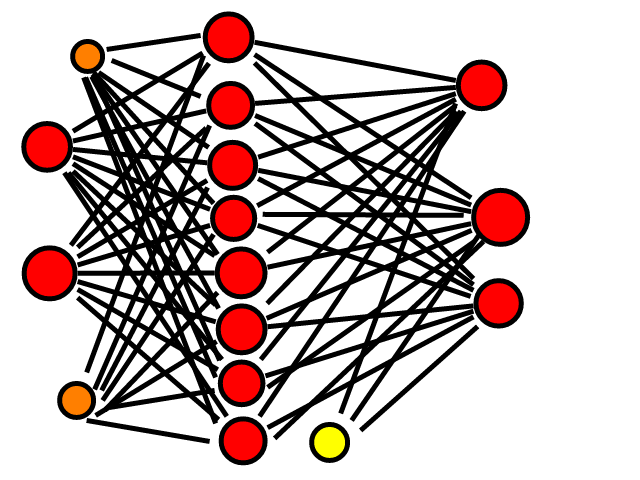
\includegraphics{neuralka.png}

    Kada biste morali rucno odrediti vrijednosti svih parametara upravo
zadane neuronske mreze, na koje biste ih vrijednosti postavili i zasto?
- Odgovoreno iznad.

Cime biste se vodili prilikom odredivanja parametara neurona skrivenog
sloja, a cime prilikom odreživanja parametara neurona izlaznog sloja? -
Takoder odgovoreno u prethodnoj kartici.

    \subsubsection{Zadatak 4.}\label{zadatak-4.}

    \begin{Verbatim}[commandchars=\\\{\}]
{\color{incolor}In [{\color{incolor}24}]:} \PY{n}{weights} \PY{o}{=}\PY{n}{np}\PY{o}{.}\PY{n}{array}\PY{p}{(}\PY{p}{[}\PY{l+m+mf}{0.6318113514388014}\PY{p}{,} \PY{o}{\PYZhy{}}\PY{l+m+mf}{0.19129343719401104}\PY{p}{,} \PY{l+m+mf}{0.24177895910559222}\PY{p}{,} \PY{o}{\PYZhy{}}\PY{l+m+mf}{0.120114428144885}\PY{p}{,} \PY{l+m+mf}{0.37374728601289525}\PY{p}{,} \PY{o}{\PYZhy{}}\PY{l+m+mf}{0.04950124768159509}\PY{p}{,} \PY{l+m+mf}{0.7592958850138558}\PY{p}{,} \PY{o}{\PYZhy{}}\PY{l+m+mf}{0.29238472956195444}\PY{p}{,} \PY{l+m+mf}{0.1161349898713811}\PY{p}{,} \PY{o}{\PYZhy{}}\PY{l+m+mf}{0.08792008650729757}\PY{p}{,} \PY{l+m+mf}{0.7500012292549865}\PY{p}{,} \PY{l+m+mf}{1.6321841123760583}\PY{p}{,} \PY{l+m+mf}{0.12492921343795796}\PY{p}{,} \PY{l+m+mf}{0.1281227935139308}\PY{p}{,} \PY{l+m+mf}{0.28206152047776406}\PY{p}{,} \PY{o}{\PYZhy{}}\PY{l+m+mf}{0.22994570277146667}\PY{p}{,} \PY{l+m+mf}{0.1250072922998301}\PY{p}{,} \PY{l+m+mf}{0.08248912241587697}\PY{p}{,} \PY{l+m+mf}{0.2564388710624792}\PY{p}{,} \PY{o}{\PYZhy{}}\PY{l+m+mf}{0.14746862126420412}\PY{p}{,} \PY{l+m+mf}{0.875011731735412}\PY{p}{,} \PY{o}{\PYZhy{}}\PY{l+m+mf}{0.13010421453481996}\PY{p}{,} \PY{l+m+mf}{0.25169563852298826}\PY{p}{,} \PY{o}{\PYZhy{}}\PY{l+m+mf}{0.2922728243398205}\PY{p}{,} \PY{l+m+mf}{0.37500650890142545}\PY{p}{,} \PY{o}{\PYZhy{}}\PY{l+m+mf}{0.1978721980813904}\PY{p}{,} \PY{l+m+mf}{0.2532256374219651}\PY{p}{,} \PY{l+m+mf}{0.13737687517521432}\PY{p}{,} \PY{l+m+mf}{0.8796217505264777}\PY{p}{,} \PY{o}{\PYZhy{}}\PY{l+m+mf}{0.07291573251077853}\PY{p}{,} \PY{l+m+mf}{0.7499786977026662}\PY{p}{,} \PY{l+m+mf}{0.5581368136707527}\PY{p}{,} \PY{o}{\PYZhy{}}\PY{l+m+mf}{76.55689956887473}\PY{p}{,} \PY{o}{\PYZhy{}}\PY{l+m+mf}{55.97475189138155}\PY{p}{,} \PY{o}{\PYZhy{}}\PY{l+m+mf}{77.57350869823716}\PY{p}{,} \PY{l+m+mf}{48.14578466068903}\PY{p}{,} \PY{l+m+mf}{43.45550027667159}\PY{p}{,} \PY{l+m+mf}{72.58606739999662}\PY{p}{,} \PY{o}{\PYZhy{}}\PY{l+m+mf}{38.13846521457862}\PY{p}{,} \PY{o}{\PYZhy{}}\PY{l+m+mf}{91.05572246579257}\PY{p}{,} \PY{l+m+mf}{41.440337686445396}\PY{p}{,} \PY{o}{\PYZhy{}}\PY{l+m+mf}{50.956614234004356}\PY{p}{,} \PY{o}{\PYZhy{}}\PY{l+m+mf}{21.08153541953472}\PY{p}{,} \PY{l+m+mf}{77.06508449438691}\PY{p}{,} \PY{o}{\PYZhy{}}\PY{l+m+mf}{41.95168920674712}\PY{p}{,} \PY{o}{\PYZhy{}}\PY{l+m+mf}{69.37474824816529}\PY{p}{,} \PY{o}{\PYZhy{}}\PY{l+m+mf}{51.077962550079235}\PY{p}{,} \PY{l+m+mf}{115.83449609358216}\PY{p}{,} \PY{l+m+mf}{74.94817719665426}\PY{p}{,} \PY{o}{\PYZhy{}}\PY{l+m+mf}{20.12508225211332}\PY{p}{,} \PY{l+m+mf}{122.54122399038398}\PY{p}{,} \PY{l+m+mf}{73.4021267744125}\PY{p}{,} \PY{l+m+mf}{9.400390520334922}\PY{p}{,} \PY{o}{\PYZhy{}}\PY{l+m+mf}{33.77656594553332}\PY{p}{,} \PY{o}{\PYZhy{}}\PY{l+m+mf}{36.68075286582176}\PY{p}{,} \PY{o}{\PYZhy{}}\PY{l+m+mf}{14.706817650953836}\PY{p}{,} \PY{o}{\PYZhy{}}\PY{l+m+mf}{77.97994420702034}\PY{p}{,} \PY{o}{\PYZhy{}}\PY{l+m+mf}{77.16294911620393}\PY{p}{,} \PY{o}{\PYZhy{}}\PY{l+m+mf}{5.426321118599951}\PY{p}{]}\PY{p}{)} 
\end{Verbatim}

    \begin{Verbatim}[commandchars=\\\{\}]
{\color{incolor}In [{\color{incolor}26}]:} \PY{n}{plt}\PY{o}{.}\PY{n}{scatter}\PY{p}{(}\PY{n}{X}\PY{p}{[}\PY{p}{:}\PY{p}{,}\PY{l+m+mi}{0}\PY{p}{]}\PY{p}{,}\PY{n}{X}\PY{p}{[}\PY{p}{:}\PY{p}{,}\PY{l+m+mi}{1}\PY{p}{]}\PY{p}{,}\PY{n}{c}\PY{o}{=}\PY{n}{cm}\PY{o}{.}\PY{n}{hot}\PY{p}{(}\PY{n}{np}\PY{o}{.}\PY{n}{argmax}\PY{p}{(}\PY{n}{y}\PY{p}{,}\PY{n}{axis}\PY{o}{=}\PY{l+m+mi}{1}\PY{p}{)}\PY{o}{*}\PY{l+m+mf}{0.5}\PY{p}{)}\PY{p}{)}\PY{p}{;}
         \PY{n}{plt}\PY{o}{.}\PY{n}{scatter}\PY{p}{(}\PY{n}{weights}\PY{p}{[}\PY{n}{np}\PY{o}{.}\PY{n}{array}\PY{p}{(}\PY{n}{np}\PY{o}{.}\PY{n}{arange}\PY{p}{(}\PY{l+m+mi}{0}\PY{p}{,}\PY{l+m+mi}{8}\PY{o}{*}\PY{l+m+mi}{4}\PY{p}{,}\PY{l+m+mi}{4}\PY{p}{)}\PY{p}{)}\PY{p}{]}\PY{p}{,}\PY{n}{weights}\PY{p}{[}\PY{n}{np}\PY{o}{.}\PY{n}{array}\PY{p}{(}\PY{n}{np}\PY{o}{.}\PY{n}{arange}\PY{p}{(}\PY{l+m+mi}{2}\PY{p}{,}\PY{l+m+mi}{8}\PY{o}{*}\PY{l+m+mi}{4}\PY{p}{,}\PY{l+m+mi}{4}\PY{p}{)}\PY{p}{)}\PY{p}{]}\PY{p}{)}\PY{p}{;}
\end{Verbatim}

    \begin{center}
    \adjustimage{max size={0.9\linewidth}{0.9\paperheight}}{neki kao grafovi_files/neki kao grafovi_15_0.png}
    \end{center}
    { \hspace*{\fill} \\}
    
    Kakve je vrijednosti parametara si naucio GA? - ocekivane

Jesu li iste za x i y komponentu ili su razlicite? - razlicite su

Uocavate li kakvu pravilnost u tim tezinama? - uocavam vec u prethodnom
zadatku

Mozete li je objasniti? - objasnjena je vec u prethodnom zadatku

    \subsubsection{Zadatak 5.}\label{zadatak-5.}

    \begin{Verbatim}[commandchars=\\\{\}]
{\color{incolor}In [{\color{incolor}30}]:} \PY{n}{weights} \PY{o}{=}\PY{n}{np}\PY{o}{.}\PY{n}{array}\PY{p}{(}\PY{p}{[}\PY{l+m+mf}{0.6190177098527958}\PY{p}{,} \PY{o}{\PYZhy{}}\PY{l+m+mf}{0.16906742020182414}\PY{p}{,} \PY{l+m+mf}{0.7485858287149564}\PY{p}{,} \PY{o}{\PYZhy{}}\PY{l+m+mf}{0.8530216626340182}\PY{p}{,} \PY{l+m+mf}{0.6285174747580695}\PY{p}{,} \PY{o}{\PYZhy{}}\PY{l+m+mf}{0.09720179017297065}\PY{p}{,} \PY{l+m+mf}{0.25227761159109985}\PY{p}{,} \PY{l+m+mf}{0.21836445182960726}\PY{p}{,} \PY{l+m+mf}{0.3896559881650747}\PY{p}{,} \PY{o}{\PYZhy{}}\PY{l+m+mf}{0.08993226473998384}\PY{p}{,} \PY{l+m+mf}{0.259107050981476}\PY{p}{,} \PY{o}{\PYZhy{}}\PY{l+m+mf}{0.16056369111146357}\PY{p}{,} \PY{l+m+mf}{0.12065346747837526}\PY{p}{,} \PY{l+m+mf}{0.1455087543269176}\PY{p}{,} \PY{l+m+mf}{0.1815735774008551}\PY{p}{,} \PY{o}{\PYZhy{}}\PY{l+m+mf}{0.4949288428625677}\PY{p}{,} \PY{l+m+mf}{0.01488564455683741}\PY{p}{,} \PY{l+m+mf}{0.200076599463153}\PY{p}{,} \PY{l+m+mf}{0.7132467312812526}\PY{p}{,} \PY{o}{\PYZhy{}}\PY{l+m+mf}{0.0725036020855885}\PY{p}{,} \PY{l+m+mf}{0.4061283802878219}\PY{p}{,} \PY{l+m+mf}{0.07161168967965546}\PY{p}{,} \PY{l+m+mf}{0.7497521226147054}\PY{p}{,} \PY{o}{\PYZhy{}}\PY{l+m+mf}{0.1957251838991895}\PY{p}{,} \PY{l+m+mf}{0.34881655236355585}\PY{p}{,} \PY{l+m+mf}{0.05864334353591021}\PY{p}{,} \PY{l+m+mf}{0.7706464063063467}\PY{p}{,} \PY{o}{\PYZhy{}}\PY{l+m+mf}{0.23308298675283828}\PY{p}{,} \PY{l+m+mf}{0.8798113744369004}\PY{p}{,} \PY{l+m+mf}{0.3139045438061595}\PY{p}{,} \PY{l+m+mf}{0.2538223305666321}\PY{p}{,} \PY{o}{\PYZhy{}}\PY{l+m+mf}{0.09394125189153629}\PY{p}{,} \PY{l+m+mf}{2.937479697571683}\PY{p}{,} \PY{l+m+mf}{3.7723547671557913}\PY{p}{,} \PY{o}{\PYZhy{}}\PY{l+m+mf}{9.295328764323747}\PY{p}{,} \PY{l+m+mf}{6.420672543636826}\PY{p}{,} \PY{o}{\PYZhy{}}\PY{l+m+mf}{4.56086761031272}\PY{p}{,} \PY{l+m+mf}{6.014949272969859}\PY{p}{,} \PY{l+m+mf}{4.0129610404862985}\PY{p}{,} \PY{l+m+mf}{4.579771985442985}\PY{p}{,} \PY{o}{\PYZhy{}}\PY{l+m+mf}{3.5473240411585616}\PY{p}{,} \PY{o}{\PYZhy{}}\PY{l+m+mf}{5.865707281194505}\PY{p}{,} \PY{l+m+mf}{12.70373501646802}\PY{p}{,} \PY{o}{\PYZhy{}}\PY{l+m+mf}{2.951700789900933}\PY{p}{,} \PY{o}{\PYZhy{}}\PY{l+m+mf}{3.9269078840803266}\PY{p}{,} \PY{l+m+mf}{0.27058609712854065}\PY{p}{,} \PY{l+m+mf}{4.062722386130711}\PY{p}{,} \PY{l+m+mf}{6.235602385549833}\PY{p}{,} \PY{o}{\PYZhy{}}\PY{l+m+mf}{3.142456054302144}\PY{p}{,} \PY{o}{\PYZhy{}}\PY{l+m+mf}{1.140014856297884}\PY{p}{,} \PY{l+m+mf}{4.648959696763723}\PY{p}{,} \PY{o}{\PYZhy{}}\PY{l+m+mf}{5.1478103870716705}\PY{p}{,} \PY{o}{\PYZhy{}}\PY{l+m+mf}{10.937137289302466}\PY{p}{,} \PY{l+m+mf}{5.90635781872721}\PY{p}{,} \PY{o}{\PYZhy{}}\PY{l+m+mf}{6.165871734319028}\PY{p}{,} \PY{l+m+mf}{0.8731979504291547}\PY{p}{,} \PY{o}{\PYZhy{}}\PY{l+m+mf}{0.9129598738157384}\PY{p}{,} \PY{l+m+mf}{3.549754630206052}\PY{p}{,} \PY{o}{\PYZhy{}}\PY{l+m+mf}{0.14174985539001408}\PY{p}{,} \PY{o}{\PYZhy{}}\PY{l+m+mf}{1.5668306890418358}\PY{p}{,} \PY{o}{\PYZhy{}}\PY{l+m+mf}{10.412399075056149}\PY{p}{,} \PY{l+m+mf}{9.519028582733398}\PY{p}{,} \PY{o}{\PYZhy{}}\PY{l+m+mf}{4.05193452476273}\PY{p}{,} \PY{l+m+mf}{9.198161783209347}\PY{p}{,} \PY{o}{\PYZhy{}}\PY{l+m+mf}{6.744832080292289}\PY{p}{,} \PY{o}{\PYZhy{}}\PY{l+m+mf}{4.480048302144393}\PY{p}{,} \PY{o}{\PYZhy{}}\PY{l+m+mf}{5.011421226112099}\PY{p}{,} \PY{l+m+mf}{3.0717582659846547}\PY{p}{,} \PY{l+m+mf}{6.565715961230712}\PY{p}{,} \PY{o}{\PYZhy{}}\PY{l+m+mf}{21.32034316850589}\PY{p}{,} \PY{l+m+mf}{18.647593114763346}\PY{p}{,} \PY{o}{\PYZhy{}}\PY{l+m+mf}{24.11255453329678}\PY{p}{,} \PY{o}{\PYZhy{}}\PY{l+m+mf}{0.932440900772823}\PY{p}{,} \PY{o}{\PYZhy{}}\PY{l+m+mf}{17.042871489327425}\PY{p}{,} \PY{o}{\PYZhy{}}\PY{l+m+mf}{1.2328601241489194}\PY{p}{,} \PY{o}{\PYZhy{}}\PY{l+m+mf}{7.7687962890334274}\PY{p}{,} \PY{l+m+mf}{23.111614540284073}\PY{p}{,} \PY{l+m+mf}{4.682283847842265}\PY{p}{,} \PY{l+m+mf}{6.214812817939961}\PY{p}{,} \PY{l+m+mf}{16.365775345186638}\PY{p}{,} \PY{o}{\PYZhy{}}\PY{l+m+mf}{12.143422110986721}\PY{p}{,} \PY{o}{\PYZhy{}}\PY{l+m+mf}{14.164182625177371}\PY{p}{,} \PY{o}{\PYZhy{}}\PY{l+m+mf}{7.039606113859401}\PY{p}{]}\PY{p}{)}
\end{Verbatim}

    \begin{Verbatim}[commandchars=\\\{\}]
{\color{incolor}In [{\color{incolor}31}]:} \PY{n}{plt}\PY{o}{.}\PY{n}{scatter}\PY{p}{(}\PY{n}{X}\PY{p}{[}\PY{p}{:}\PY{p}{,}\PY{l+m+mi}{0}\PY{p}{]}\PY{p}{,}\PY{n}{X}\PY{p}{[}\PY{p}{:}\PY{p}{,}\PY{l+m+mi}{1}\PY{p}{]}\PY{p}{,}\PY{n}{c}\PY{o}{=}\PY{n}{cm}\PY{o}{.}\PY{n}{hot}\PY{p}{(}\PY{n}{np}\PY{o}{.}\PY{n}{argmax}\PY{p}{(}\PY{n}{y}\PY{p}{,}\PY{n}{axis}\PY{o}{=}\PY{l+m+mi}{1}\PY{p}{)}\PY{o}{*}\PY{l+m+mf}{0.5}\PY{p}{)}\PY{p}{)}\PY{p}{;}
         \PY{n}{plt}\PY{o}{.}\PY{n}{scatter}\PY{p}{(}\PY{n}{weights}\PY{p}{[}\PY{n}{np}\PY{o}{.}\PY{n}{array}\PY{p}{(}\PY{n}{np}\PY{o}{.}\PY{n}{arange}\PY{p}{(}\PY{l+m+mi}{0}\PY{p}{,}\PY{l+m+mi}{8}\PY{o}{*}\PY{l+m+mi}{4}\PY{p}{,}\PY{l+m+mi}{4}\PY{p}{)}\PY{p}{)}\PY{p}{]}\PY{p}{,}\PY{n}{weights}\PY{p}{[}\PY{n}{np}\PY{o}{.}\PY{n}{array}\PY{p}{(}\PY{n}{np}\PY{o}{.}\PY{n}{arange}\PY{p}{(}\PY{l+m+mi}{2}\PY{p}{,}\PY{l+m+mi}{8}\PY{o}{*}\PY{l+m+mi}{4}\PY{p}{,}\PY{l+m+mi}{4}\PY{p}{)}\PY{p}{)}\PY{p}{]}\PY{p}{)}\PY{p}{;}
\end{Verbatim}

    \begin{center}
    \adjustimage{max size={0.9\linewidth}{0.9\paperheight}}{neki kao grafovi_files/neki kao grafovi_19_0.png}
    \end{center}
    { \hspace*{\fill} \\}
    
    Je li postupak ucenja trajao dulje ili krace u odnosu na prethodnu
arhitekturu? - krace

Mozete li objasniti zasto? - mogu, model je slozeniji pa je lakse
prenauci jednostavnije modele

Pogledajte naucene parametre u neuronima tipa 1 za ovaj slucaj. Mozete
li ih objasniti? - ne mogu bez poznavanja parametra drugog sloja

    \subsubsection{Zadatak 6.}\label{zadatak-6.}

    \begin{Verbatim}[commandchars=\\\{\}]
{\color{incolor}In [{\color{incolor}32}]:} \PY{n}{weights} \PY{o}{=}\PY{n}{np}\PY{o}{.}\PY{n}{array}\PY{p}{(}\PY{p}{[}\PY{l+m+mf}{0.08290295394240876}\PY{p}{,} \PY{l+m+mf}{0.06451709135948638}\PY{p}{,} \PY{l+m+mf}{0.7688391605977419}\PY{p}{,} \PY{o}{\PYZhy{}}\PY{l+m+mf}{0.1432605506959392}\PY{p}{,} \PY{l+m+mf}{0.12697309234753767}\PY{p}{,} \PY{l+m+mf}{0.05580754743331135}\PY{p}{,} \PY{l+m+mf}{0.3516290438914602}\PY{p}{,} \PY{o}{\PYZhy{}}\PY{l+m+mf}{0.05577272333750271}\PY{p}{,} \PY{l+m+mf}{0.3000837817484028}\PY{p}{,} \PY{l+m+mf}{0.04937250982845218}\PY{p}{,} \PY{l+m+mf}{0.6394351992535006}\PY{p}{,} \PY{o}{\PYZhy{}}\PY{l+m+mf}{0.4126108630334583}\PY{p}{,} \PY{l+m+mf}{0.42049694175624674}\PY{p}{,} \PY{l+m+mf}{0.16155910082725672}\PY{p}{,} \PY{l+m+mf}{0.24973831800412102}\PY{p}{,} \PY{o}{\PYZhy{}}\PY{l+m+mf}{0.25819472641319496}\PY{p}{,} \PY{l+m+mf}{0.5589618063692977}\PY{p}{,} \PY{l+m+mf}{0.08022064872999946}\PY{p}{,} \PY{l+m+mf}{0.7294107019389107}\PY{p}{,} \PY{l+m+mf}{0.4371962928630494}\PY{p}{,} \PY{l+m+mf}{0.02545018590842006}\PY{p}{,} \PY{l+m+mf}{23.53128414350101}\PY{p}{,} \PY{l+m+mf}{0.22902768438240964}\PY{p}{,} \PY{l+m+mf}{0.2124648714881792}\PY{p}{,} \PY{o}{\PYZhy{}}\PY{l+m+mf}{2.7913501617751666}\PY{p}{,} \PY{l+m+mf}{16.73426224222317}\PY{p}{,} \PY{o}{\PYZhy{}}\PY{l+m+mf}{0.4427953561314091}\PY{p}{,} \PY{o}{\PYZhy{}}\PY{l+m+mf}{10.002476994056652}\PY{p}{,} \PY{o}{\PYZhy{}}\PY{l+m+mf}{19.534821022396}\PY{p}{,} \PY{l+m+mf}{7.216913073462565}\PY{p}{,} \PY{l+m+mf}{0.7396188072031955}\PY{p}{,} \PY{l+m+mf}{5.712608323579977}\PY{p}{,} \PY{l+m+mf}{7.8259142916701325}\PY{p}{,} \PY{l+m+mf}{14.712506314205166}\PY{p}{,} \PY{l+m+mf}{14.062301352444255}\PY{p}{,} \PY{o}{\PYZhy{}}\PY{l+m+mf}{10.380688183904578}\PY{p}{,} \PY{l+m+mf}{3.1902740740194164}\PY{p}{,} \PY{o}{\PYZhy{}}\PY{l+m+mf}{5.155560249832584}\PY{p}{,} \PY{l+m+mf}{7.090035386718857}\PY{p}{,} \PY{o}{\PYZhy{}}\PY{l+m+mf}{6.272496767673904}\PY{p}{,} \PY{o}{\PYZhy{}}\PY{l+m+mf}{3.96163829738354}\PY{p}{,} \PY{l+m+mf}{11.957127568504452}\PY{p}{,} \PY{o}{\PYZhy{}}\PY{l+m+mf}{10.993272481498026}\PY{p}{,} \PY{o}{\PYZhy{}}\PY{l+m+mf}{1.2150471486327448}\PY{p}{,} \PY{l+m+mf}{0.4840806961806887}\PY{p}{,} \PY{l+m+mf}{5.945528108663184}\PY{p}{,} \PY{o}{\PYZhy{}}\PY{l+m+mf}{1.0603215143730564}\PY{p}{,} \PY{o}{\PYZhy{}}\PY{l+m+mf}{2.4512857879469214}\PY{p}{,} \PY{l+m+mf}{10.001524872443502}\PY{p}{,} \PY{o}{\PYZhy{}}\PY{l+m+mf}{13.530306421734409}\PY{p}{,} \PY{o}{\PYZhy{}}\PY{l+m+mf}{3.1817811657751203}\PY{p}{,} \PY{l+m+mf}{1.1501103663878536}\PY{p}{,} \PY{l+m+mf}{50.62723530189632}\PY{p}{,} \PY{o}{\PYZhy{}}\PY{l+m+mf}{13.34978849863527}\PY{p}{,} \PY{o}{\PYZhy{}}\PY{l+m+mf}{27.12238360570009}\PY{p}{,} \PY{o}{\PYZhy{}}\PY{l+m+mf}{31.49463338406667}\PY{p}{,} \PY{l+m+mf}{14.194374973105482}\PY{p}{,} \PY{o}{\PYZhy{}}\PY{l+m+mf}{18.335795255511712}\PY{p}{,} \PY{o}{\PYZhy{}}\PY{l+m+mf}{26.807412008428418}\PY{p}{,} \PY{l+m+mf}{25.76881912301195}\PY{p}{,} \PY{l+m+mf}{41.00283013391715}\PY{p}{,} \PY{o}{\PYZhy{}}\PY{l+m+mf}{12.388211064314012}\PY{p}{,} \PY{o}{\PYZhy{}}\PY{l+m+mf}{20.132364897336206}\PY{p}{,} \PY{l+m+mf}{30.18539451529129}\PY{p}{,} \PY{o}{\PYZhy{}}\PY{l+m+mf}{1.9649920657391016}\PY{p}{,} \PY{o}{\PYZhy{}}\PY{l+m+mf}{31.812050236854837}\PY{p}{,} \PY{o}{\PYZhy{}}\PY{l+m+mf}{8.381825336226948}\PY{p}{]}\PY{p}{)}
\end{Verbatim}

    \begin{Verbatim}[commandchars=\\\{\}]
{\color{incolor}In [{\color{incolor}33}]:} \PY{n}{plt}\PY{o}{.}\PY{n}{scatter}\PY{p}{(}\PY{n}{X}\PY{p}{[}\PY{p}{:}\PY{p}{,}\PY{l+m+mi}{0}\PY{p}{]}\PY{p}{,}\PY{n}{X}\PY{p}{[}\PY{p}{:}\PY{p}{,}\PY{l+m+mi}{1}\PY{p}{]}\PY{p}{,}\PY{n}{c}\PY{o}{=}\PY{n}{cm}\PY{o}{.}\PY{n}{hot}\PY{p}{(}\PY{n}{np}\PY{o}{.}\PY{n}{argmax}\PY{p}{(}\PY{n}{y}\PY{p}{,}\PY{n}{axis}\PY{o}{=}\PY{l+m+mi}{1}\PY{p}{)}\PY{o}{*}\PY{l+m+mf}{0.5}\PY{p}{)}\PY{p}{)}\PY{p}{;}
         \PY{n}{plt}\PY{o}{.}\PY{n}{scatter}\PY{p}{(}\PY{n}{weights}\PY{p}{[}\PY{n}{np}\PY{o}{.}\PY{n}{array}\PY{p}{(}\PY{n}{np}\PY{o}{.}\PY{n}{arange}\PY{p}{(}\PY{l+m+mi}{0}\PY{p}{,}\PY{l+m+mi}{8}\PY{o}{*}\PY{l+m+mi}{4}\PY{p}{,}\PY{l+m+mi}{4}\PY{p}{)}\PY{p}{)}\PY{p}{]}\PY{p}{,}\PY{n}{weights}\PY{p}{[}\PY{n}{np}\PY{o}{.}\PY{n}{array}\PY{p}{(}\PY{n}{np}\PY{o}{.}\PY{n}{arange}\PY{p}{(}\PY{l+m+mi}{2}\PY{p}{,}\PY{l+m+mi}{8}\PY{o}{*}\PY{l+m+mi}{4}\PY{p}{,}\PY{l+m+mi}{4}\PY{p}{)}\PY{p}{)}\PY{p}{]}\PY{p}{)}\PY{p}{;}
\end{Verbatim}

    \begin{center}
    \adjustimage{max size={0.9\linewidth}{0.9\paperheight}}{neki kao grafovi_files/neki kao grafovi_23_0.png}
    \end{center}
    { \hspace*{\fill} \\}
    
 Mozete li dobiti ispravnu klasifkaciju svih uzoraka u arhitekturi koja
ima N1 \textless{} 8 ? Provjerite to na arhitekturi 2×6×4×3. - mogu

Na kraju (uspjesnog ili neuspjesnog) postupka ucenja pogledajte za
najbolje rjesenje parametre u neuronima tipa 1 za ovaj slucaj. ’Sto smo
izgubili u odnosu na mrezu iz zadatka 4? - interpretabilnost


    % Add a bibliography block to the postdoc
    
    
    
    \end{document}
